\chapter{Calculations}

\section{Structural}

The steel sheets that make up the shell of the Notchmatic require a minimum length of thread engagement in order to fit securely. To calculate this length, the equation below is used. In the equation, At is Thread Tensile Stress Area, Knmax is Maximum Minor Diameter Internal Thread, Esmin is Minimum Pitch Diameter External Thread, and n is the Threads per Inch. 

\begin{figure}[H]
    \centering
    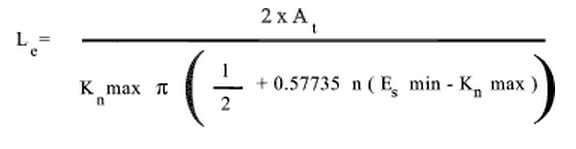
\includegraphics[width=0.6\textwidth]{./fall-report pictures/Chapter3-Calculations/ShellThread}
    \label{fig:ThreadEng}
\end{figure}

Fastener thread engagement length for a 8-32 bolt is 0.140 inches. The head stock frame thickness is 0.12 inches. Although, the head stock frame thickness is 0.02 inches less than the require fastener thread engagement length, the head stock frame does not experience any significant load during cutting operations. 

\newpage

The following is a calculation of the effects of vibration on the Motor Mount of the AC Spindle Drive Motor. ANSYS Mechanical was used and the frequency at the first 6 modes were found. The rpm of the driveline motor is 1750, and the natural frequency of the motor mount is over 2000.

\begin{figure}[H]
    \centering
    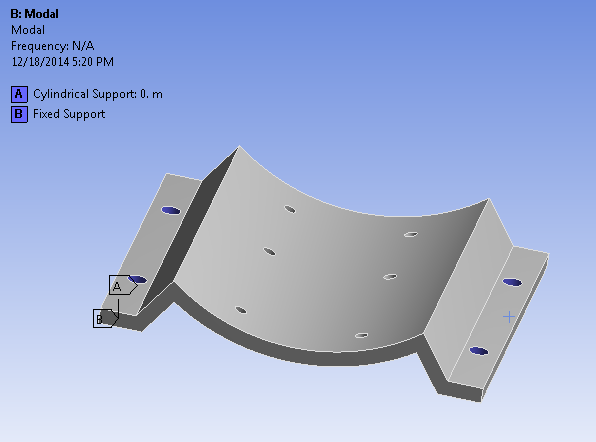
\includegraphics[width=0.6\textwidth]{./fall-report pictures/Chapter3-Calculations/AnsysMotorMount}
    \label{fig:MM1}
\end{figure}

\begin{figure}[H]
    \centering
    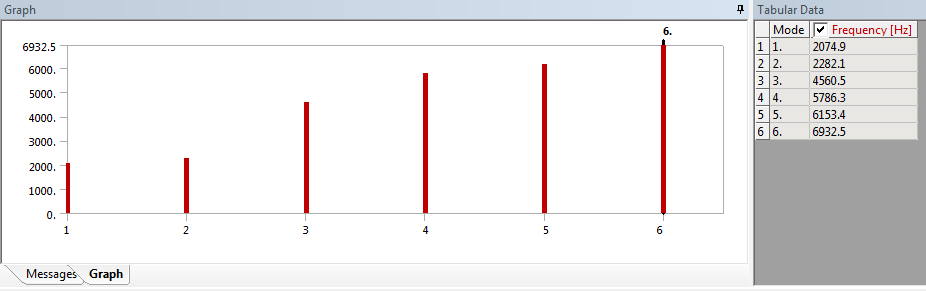
\includegraphics[width=0.6\textwidth]{./fall-report pictures/Chapter3-Calculations/AnsysMotorMount2}
    \label{fig:MM2}
\end{figure}

\newpage

An ANSYS FEA Analysis was conducted earlier in the design in the frame. Since that esign iteration, the base structure of the frame has not changed dramatically. For that reason, it was concluded that the frame's current design, sufficiently bears the forces that the machine will experience during operation. Below is the results of the earlier simulation.

In total 8 loads, labeled C to J, were applied to the frame. Loads C and D represent the weight of the spindle motor and transformer. Load E represents the weight of an individual leaning on the machine while it is in use.  Loads F,G,H, and I represent forces that are generated when a piece is being machined. Lastly, Load J represents the weight of the aluminum headstock and the driveline assembly. 

\begin{figure}[H]
    \centering
    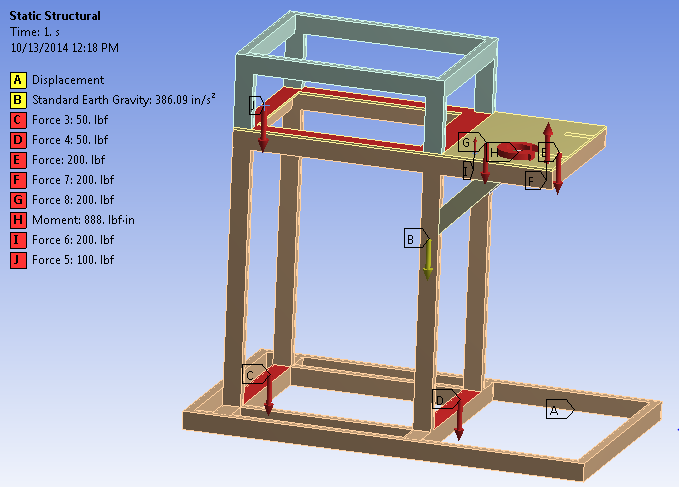
\includegraphics[width=0.8\textwidth]{./fall-report pictures/Chapter3-Calculations/lp1}
    \label{fig:MM2}
\end{figure}

\begin{figure}[H]
    \centering
    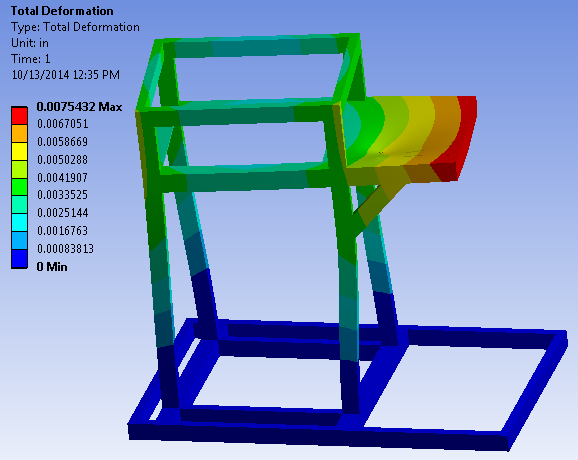
\includegraphics[width=0.6\textwidth]{./fall-report pictures/Chapter3-Calculations/mp1}
    \label{fig:MM2}
\end{figure}

\begin{figure}[H]
    \centering
    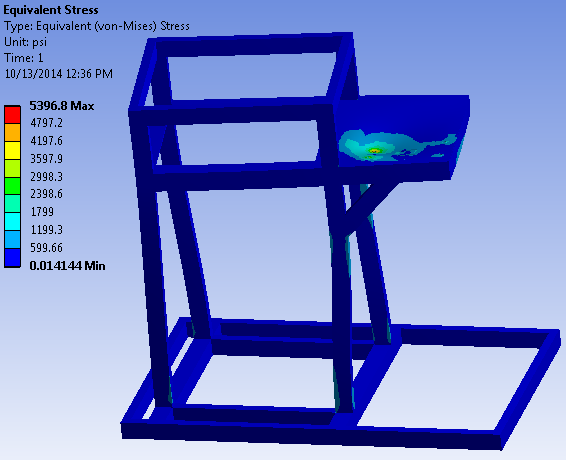
\includegraphics[width=0.6\textwidth]{./fall-report pictures/Chapter3-Calculations/mp2}
    \label{fig:MM2}
\end{figure}

This current test demonstrated a displacement of 6.93e-5 meters at the hanging bed’s edges (much less than the goal 1/32 inches maximum deflection of the bed) and a maximum stress of only 9.4e6 Pa. However, the model must be retested with corrected values from cutting force calculations. This current test demonstrated a displacement of 6.93e-5 meters at the hanging bed’s edges (much less than the goal 1/32 inches maximum deflection of the bed) and a maximum stress of only 9.4e6 Pa.


